\subsection{iOS Architecture Patterns}

\begin{breakbox}
\boxtitle{Model-View-Controller (MVC)}

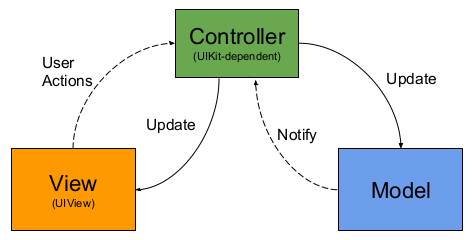
\includegraphics[width=.15\textwidth]{figures/mvc.png}

\textbf{Problems:}

\begin{itemize}
\tightlist
\item
  Tight Coupling between View and View Controller
\item
  Controller is hard to test because of UIKit dependency
\item
  MVC == Massive View Controller
\end{itemize}
\end{breakbox}

\begin{breakbox}
\boxtitle{Model-View-Presenter (MVP)}

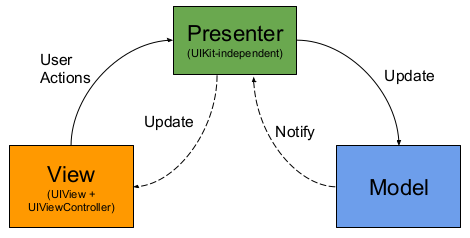
\includegraphics[width=.15\textwidth]{figures/mvp.png}

\begin{itemize}
\tightlist
\item
  Difference here is, that the ViewController is now on the View
\item
  The View knows the presenter now, but the presenter doesn't know the
  view or is loosely coupled to View via protocol.
\end{itemize}
\end{breakbox}

\begin{breakbox}
\boxtitle{Model-View-ViewModel (MVVM)}

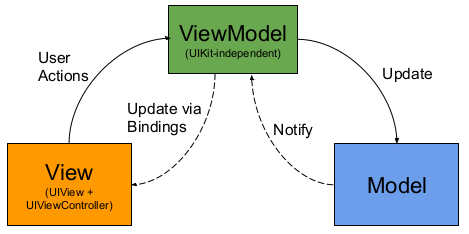
\includegraphics[width=.15\textwidth]{figures/mvvm.png}

The view

\begin{itemize}
\tightlist
\item
  Notifies ViewModel about user-actions and observes properties of
  ViewModel
\item
  Knows the ViewModel
\end{itemize}
\end{breakbox}


\subsection{Networking with URLSession}

\begin{breakbox}

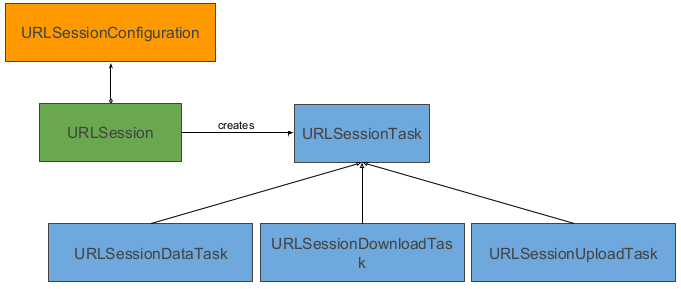
\includegraphics[width=.15\textwidth]{figures/urlSession.png}

\textbf{URLSessionConfiguration}: \\
Defines behaviour and policies

\textbf{URL}: Immutable value type to represent a URL

\textbf{URLRequest}:

\begin{itemize}
\tightlist
\item
  Wrapper around URL
\item
  Can override settings from URLSessionConfiguration
\item
  Add additional HTTP headers
\item
  Set the HTTP method (e.g., GET, PUT POST)
\item
  Set the HTTP body (e.g., JSON data)
\end{itemize}

\textbf{URLSessionTask}:

\begin{itemize}
\tightlist
\item
  A task represents a specific download / upload
\item
  Tasks are created using URLSession's factory methods
\item
  There are different subclasses of URLSessionTask:

  \begin{itemize}
  \tightlist
  \item
    URLSessionDataTask
  \item
    URLSessionUploadTask
  \item
    URLSessionDownloadTask
  \end{itemize}
\item
  All tasks start in a suspended state. Call resume() to start the task.
\item
  Completion handler is executed on background thread.
\end{itemize}
\end{breakbox}

\columnbreak
\subsection{Core Data}

\begin{breakbox}

Persistence Framework for iOS / macOS

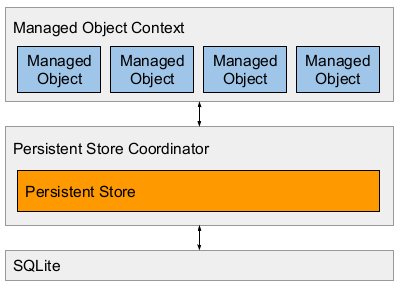
\includegraphics[width=.12\textwidth]{figures/coreData.png}

\begin{itemize}
\tightlist
\item
  As persistent store, mostly SQLite is used
\item
  Core Data takes care of the persistent store
\item
  You only have access to the managed objects, which are your models
\end{itemize}
\end{breakbox}
\begin{breakbox}
\boxtitle{Way to go}

\begin{itemize}
\tightlist
\item
  Helper class that sets up Core Data Stack
\item
  Can be passed around between view controller classes
\item
  Provides access to the managed object context
\end{itemize}

\begin{lstlisting}[language=swift]
func createOrder() {
    let order = Order(context: coreDataStack.context)
    order.uuid = UUID()
    ...
    coreDataStack.saveContext()
}
func addLineItem(beverage: Beverage, to order: Order) {
    let lineItem = LineItem(context: coreDataStack.context)
    ...
    order.addToLineItems(lineItem)
    coreDataStack.saveContext() 
}
func deleteOrders(_ orders: [Order]) {
    for order in orders { coreDataStack.context.delete(order) }
    coreDataStack.saveContext() }
\end{lstlisting}
\end{breakbox}

\begin{breakbox}
\boxtitle{Fetch Requests}

\begin{itemize}
\tightlist
\item
  Describes which data to fetch from the persistent store
\item
  Set predicate to filter results
\item
  Use Sort Descriptors to sort results
\end{itemize}

\begin{lstlisting}[language=swift]
func fetchUnfinishedOrders() -> [Order] {
    let fetchRequest: NSFetchRequest<Order> = Order.fetchRequest()
    fetchRequest.predicate = NSPredicate(format: "isFrozen == true AND isReady == false")
    return (try? coreDataStack.context.fetch(fetchRequest)) ?? []
}
\end{lstlisting}
\end{breakbox}

\subsection{Siri Shortcuts}
\begin{breakbox}

\begin{itemize}
\tightlist
\item
  Allows you to make certain actions of your app available from Siri and
  from the Shortcuts App
\item
  App ``donates'' shortcuts to the system
\item
  Siri interacts with an extension of the main app
\end{itemize}
\end{breakbox}

\subsection{Remote Notifications}
\begin{breakbox}
\begin{itemize}
\tightlist
\item
  Allows us to send a notification from our server to the devices that
  are running our app
\item
  Requires permission from the user
\item
  Notifications can be silent or they can contain a payload
\end{itemize}
\end{breakbox}

\begin{breakbox}
\boxtitle{Overview}

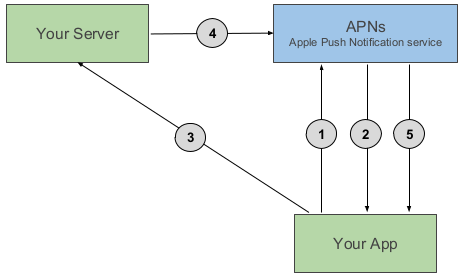
\includegraphics[width=.15\textwidth]{figures/remoteNotification.png}

\begin{enumerate}
\def\labelenumi{\arabic{enumi}.}
\tightlist
\item
  Register for remote notifications
\item
  Retrieve an app- and device specific token
\item
  Send the token to your server
\item
  When something interesting happens, your server sends a remote
  notification along with a set of tokens to APNs
\item
  APNs delivers the notification to the corresponding devices
\end{enumerate}
\end{breakbox}